\documentclass[a4j, 11pt]{jsarticle}

\usepackage[dvipdfmx]{graphicx}
\usepackage{bm}
\usepackage{amsmath}
\usepackage{amssymb}
\usepackage{amsthm} 
\usepackage{url}
\usepackage{here}

\numberwithin{equation}{section}
\renewcommand{\proofname}{\textbf{証明}}

\DeclareMathOperator*{\argmin}{argmin}
\DeclareMathOperator*{\argmax}{argmax}
\newcommand{\mathbm}[1]{{\mbox{\boldmath $#1$}}}

\title{ロジスティック回帰} 
\author{長谷川駿一}
\date{2022年5月27日 }
\begin{document}
\maketitle
\section{概要}
\indent ロジスティック回帰とは,複数の説明変数から分析を行う\textbf{多変量解析}の一種であり,二値分類(0か1か,成功か失敗か など)を行う\textbf{「分類」}に属する手法である.\\
\indent 2つの状態において,\textbf{正事象}(予測したい事象)の起こる確率を求め,一般的に確率が0.5以上なら正事象に属し,0.5未満であればもう一方の事象に属すると判定する.\\
\indent 具体例を見ていく.ある企業で,他の企業に対して訪問し,契約が成立するか成立しないかを事前に予測したいと考える.ここで,説明変数は「その企業に対しての訪問回数」としているが,他にも「資料の出来栄え」「その日の天気の具合」など,複数の要因が考えられる.目的関数は契約が成立するかしないかの二値である(図\ref{営業データ}).\\
\indent ここで,我々が予測したいのは,この営業で契約が成立する確率であり,確率は0以上1以下の値をとるため,図2のようなグラフで表現できることが想像できる(ロジスティック回帰のモデル関数(予測値を出力する関数)である\textbf{シグモイド関数}は,このような形をしている).\\

\begin{figure}[htbp]
  \begin{minipage}[b]{0.5\linewidth}
    \centering
    \mbox{\raisebox{-4mm}{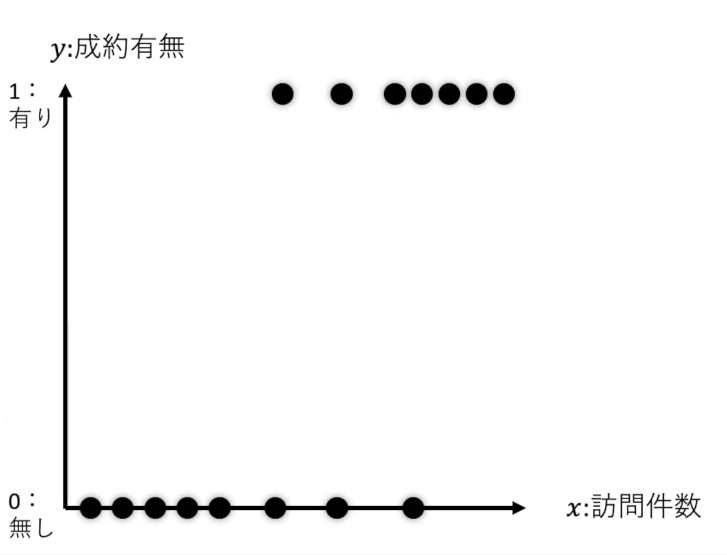
\includegraphics[scale=0.5]{fig1.png}}}
    \caption{ある企業の営業データ}
    \label{営業データ}
  \end{minipage}
  \begin{minipage}[b]{0.6\linewidth} \label{営業データ確率}
    \centering
     \vspace{5mm}
     \mbox{\raisebox{1mm}{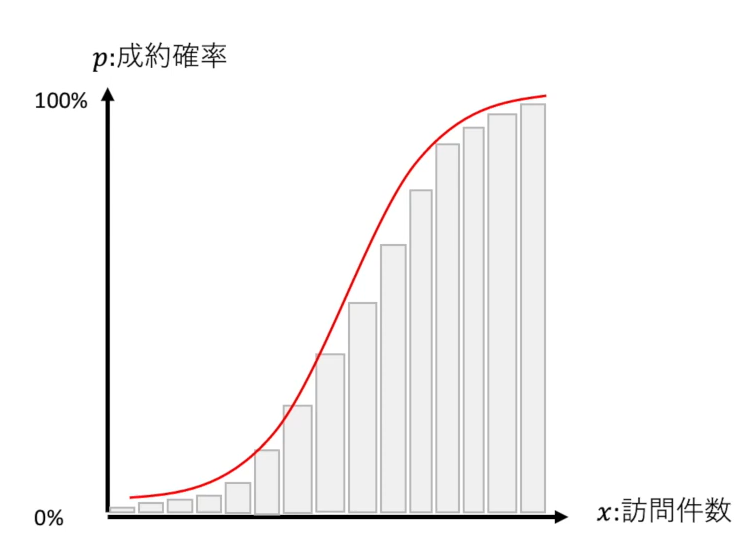
\includegraphics[scale=0.5]{fig2.png}}}
    \caption{ある企業の営業データ(確率的に表したもの)}
  \end{minipage}
\end{figure}

%% 
\section{前提知識}
%%
\subsection{シグモイド関数}
\indent ロジスティック回帰のモデル関数であるシグモイド関数を理解するために,まず\textbf{オッズ}というものを考える.オッズとは,事象の起こりやすさを表すもので,正事象の確率$p$に対して$\frac{p}{1-p}$で表すことができる.この
オッズに対して対数をとったものを\textbf{ロジット}関数と呼び,以下のように定義される.
\begin{equation}
		{\rm logit}(p) = \log{\frac{p}{(1-p)}}
 \end{equation}
\indent このロジット関数だが,図3に示すように,実数全体に対して値をとりうる.よって,特徴量の値とロジット関数との間に線形関係を表すことができる.
\begin{equation}
		{\rm logit}(p(y=1|\mathbm{x})) = w_0x_0+w_1x_1+\cdots+w_mx_m = \sum_{i=0}^{m}w_ix_i = \mathbm{w^tx}
 	\end{equation}
 	
\indent ここで,$p(y=1|\mathbm{x})$は,特徴量$\mathbm{x}$が与えられた場合にデータ点がクラス1に所属するという条件付き確率を示す($y$は分類するクラスを表し,2つに分類するため,1か0の値をとる).\\
\indent また,$w_0$は\textbf{バイアスユニット}(一次関数$y=ax+b$でいうところの切片$b$)を表し,$x_0$は1に設定される.\\

\indent シグモイド関数とは,このロジット関数の逆関数であり,総入力$z = \mathbm{w^tx}$を入力値としている.以下のように定義され,グラフを図4に示す.
\begin{equation}
		\phi (z) = \frac{1}{(1+e^{-z})}
		\label{sigmo}
 	\end{equation}
 	
\indent よってシグモイド関数は,総入力$z$を入力値,正事象(クラス1)である確率$p$を出力値とする.\\

\begin{figure}[htbp]
  \begin{minipage}[b]{0.5\linewidth}
    \centering
    \mbox{{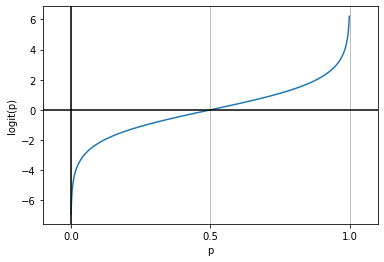
\includegraphics[scale=0.5]{fig3_logit.png}}}
    \caption{ロジット関数}
    \label{ロジット}
  \end{minipage}
  \begin{minipage}[b]{0.5\linewidth} 
    \centering
     \mbox{\raisebox{2mm}{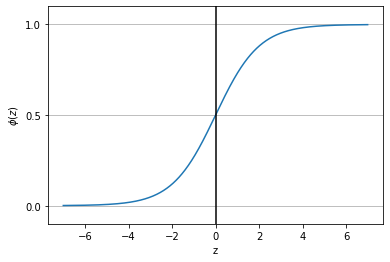
\includegraphics[scale=0.5]{fig4_sigmoid.png}}}
    \caption{シグモイド関数}
  \end{minipage}
\end{figure}

%%%
\subsection{勾配降下法(コスト関数の最小化)}
\indent 機械学習において,学習過程で最適化される\textbf{目的関数}のほとんどが,最小化したい\textbf{コスト関数}である.勾配降下法は,このコスト関数の最小値を見つける手法の一つである.\\
(ただし,コスト関数の特徴として,微分可能であること,凸関数であることが挙げられる.)\\
\indent 図5に示すように,勾配降下法は,大域的最小値に達するまで坂を下るイメージである.\\


\begin{figure}[htbp]
    \centering
    \mbox{{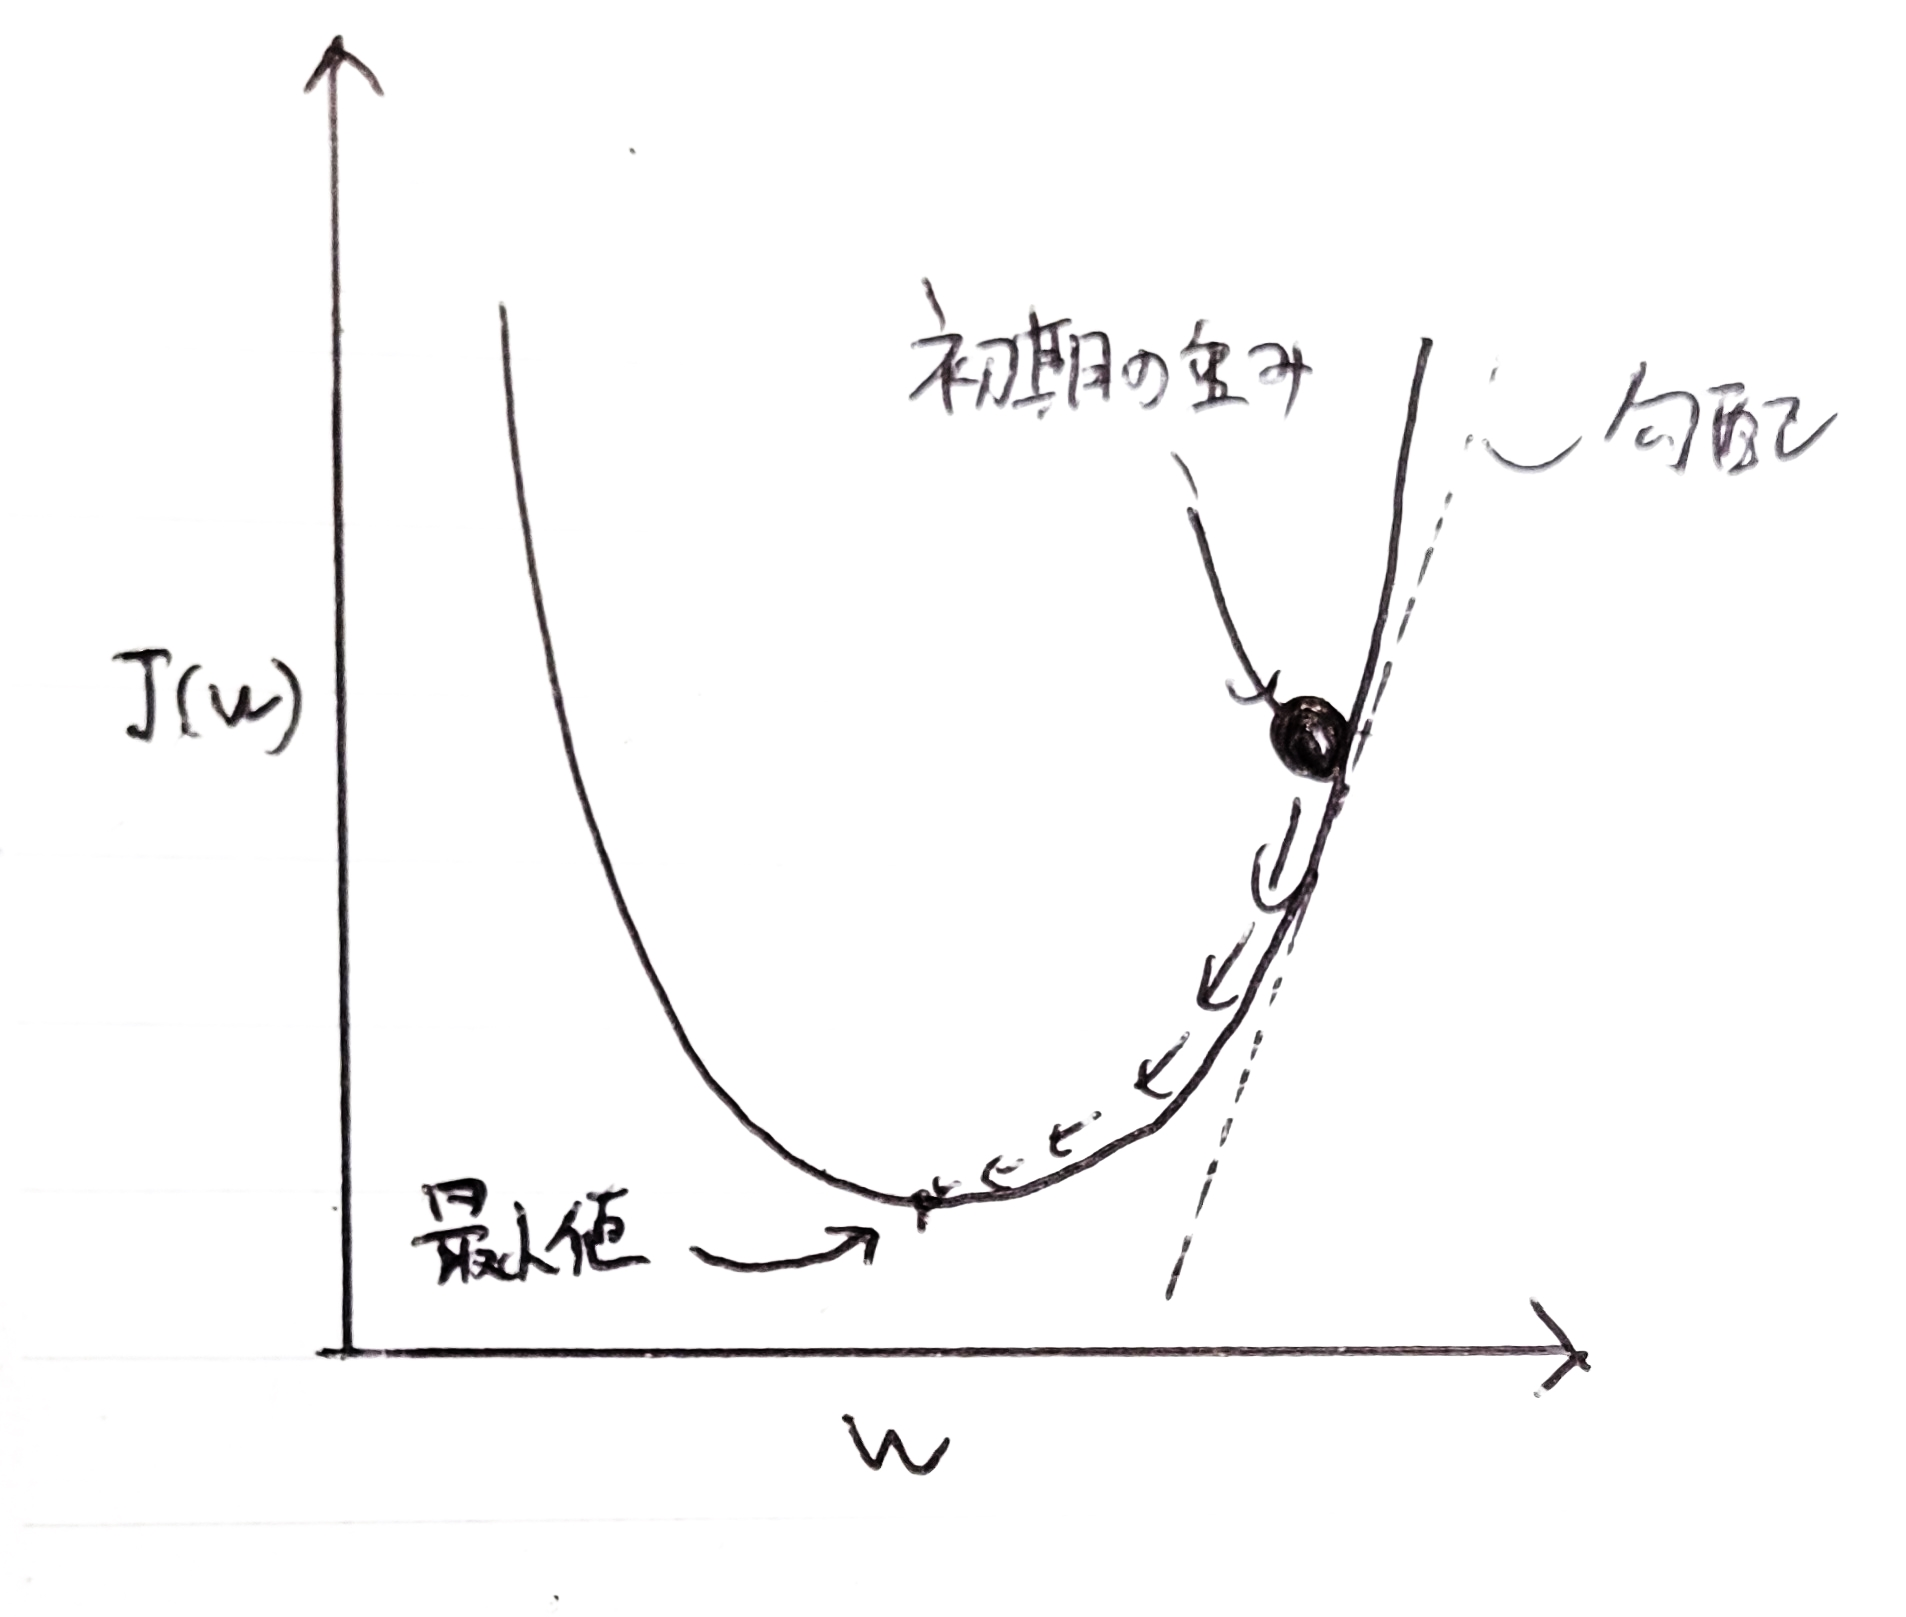
\includegraphics[scale=0.15]{fig5_gradient.jpg}}}
    \caption{勾配降下法のイメージ}
    \label{勾配}
\end{figure}

\indent 多くのモデルでは,コスト関数$J$は,以下のような\textbf{誤差平方和}で定義される.この関数は微分可能かつ凸関数であり,最小値が誤差の最小をとるので,コスト関数として適切である.\\
\begin{equation}
	J(\mathbm{w}) = \frac{1}{2}\sum_{i}\left(y^{(i)}-\hat{y}^{(i)}\right)^2
	\label{SSE}
 \end{equation}

\indent ここで,$\hat{y};\mathbm{w}$である.また,添え字$i$は,$i$番目の訓練データの真のクラスラベル$y^{(i)}$及び予測されたクラスラベル$\hat{y}^{(i)}$を表している.\\
\indent 勾配降下法を使って重みを更新するには,コスト関数$J(\mathbm{w})$の勾配$\nabla J(\mathbm{w})$に沿って動く.重みの変化である$\nabla w$は,負の勾配に\textbf{学習率}$\eta$を掛けたものとして定義される(勾配を負にするのは,重みの更新は勾配と逆方向に進むためである).\\

\begin{align} 
	\mathbm{w}&:=\mathbm{w}+\mathbm{\nabla w}\\
	\mathbm{\nabla w} &= -\eta\mathbm{\nabla J}(\mathbm{w})
\end{align}

\indent 重みの更新回数に対する措置として,以下のような方法がある.\\
\indent i)  あらかじめデータセットに対する訓練の回数(\textbf{エポック})を決める.\\
\indent ii) 重みの変化量が一定の値より小さくなったら更新をやめる.\\
\\
\indent また,学習率$\eta$は,通常は0.0よりも大きく1.0以上の定数をとる.学習率が小さすぎると,重みの更新の変化量が小さいため,コスト関数の大域的最小値に収束させるために相当な数のエポックが必要になる.また,学習率が大きすぎると,大域的最小値を超えて更新されてしまうことがあり,発散してしまう可能性がある(図6).いずれにせよ最適な学習率を設定することが重要である.\\

\begin{figure}[htbp]
    \centering
    \mbox{{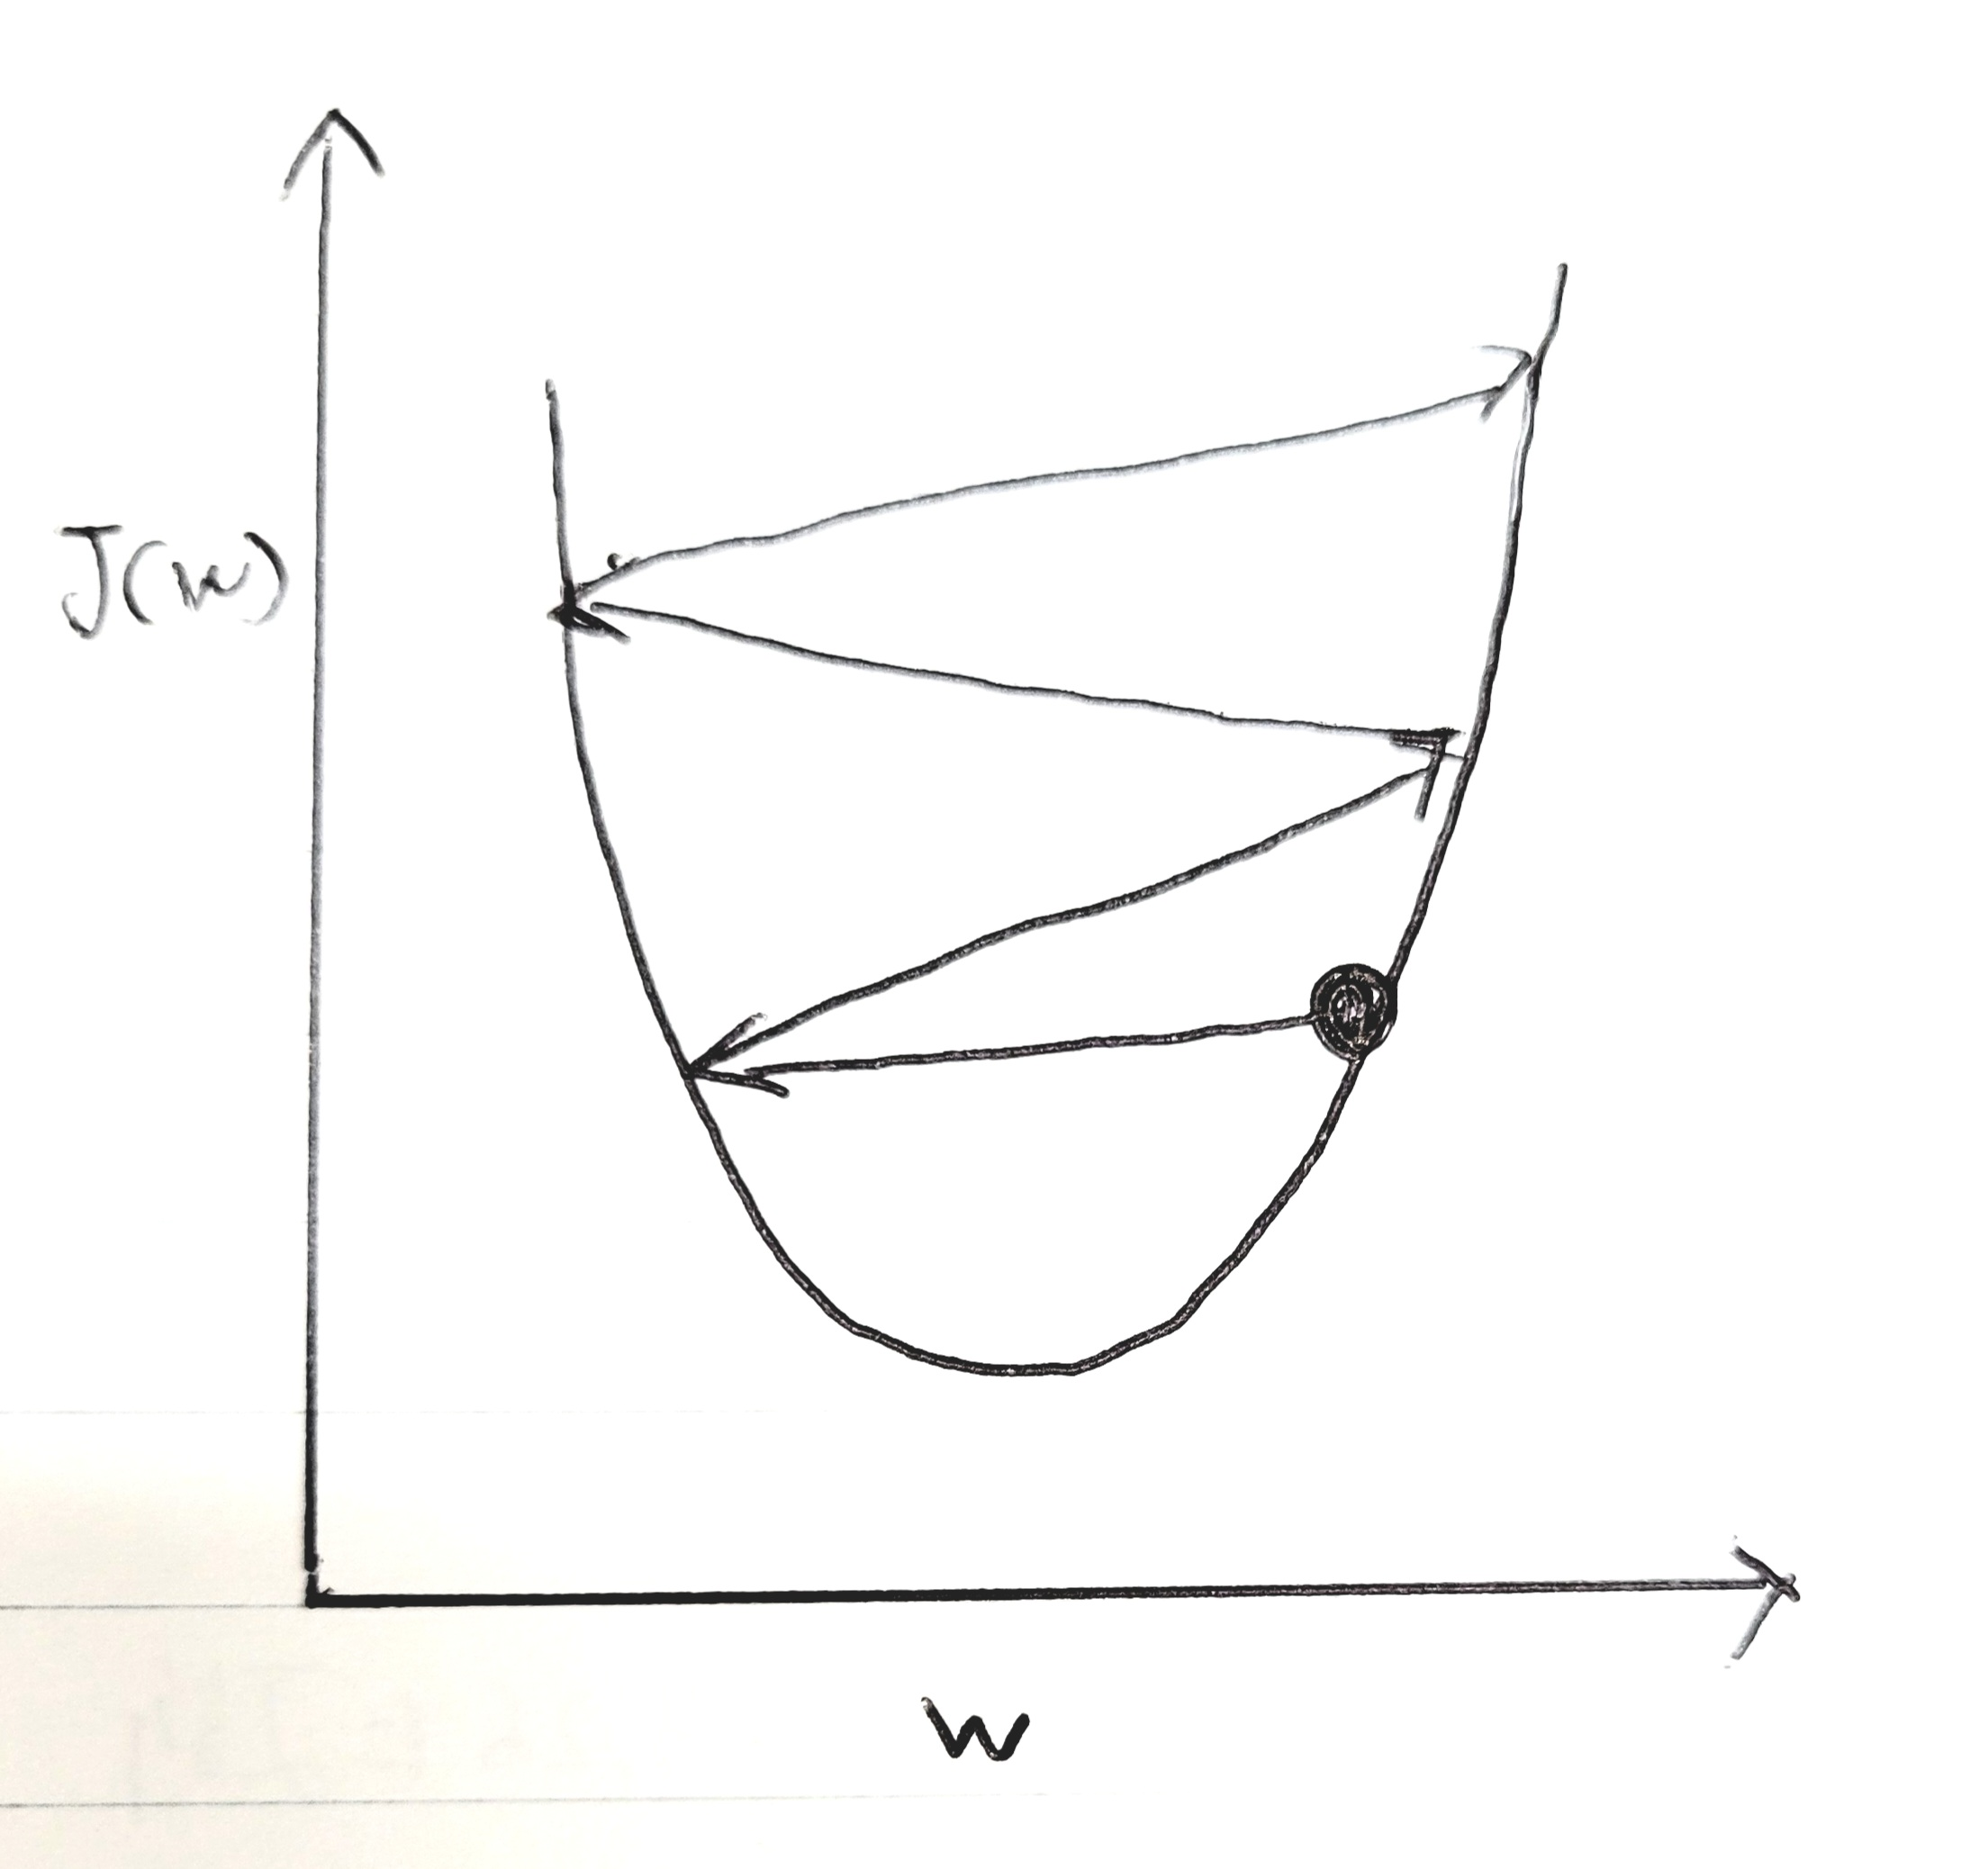
\includegraphics[scale=0.1]{fig6_grad_hassan.jpg}}}
    \caption{勾配降下法で発散する様子}
    \label{発散}
\end{figure}

\newpage

%%% 
\section{ロジスティック回帰によるモデルの構築}
\subsection{ロジスティック回帰による分類}
\indent ロジスティック回帰による予測値$\hat{y}$は,クラス1に属する確率から分類されたクラスラベルである「0」か「1」をとるため,以下のような出力値をとる.ここで,zは総入力$\mathbm{w^tx}$である.\\

\begin{equation}
	\hat{y} =   
	\begin{cases}
		1 & (\phi(z) \geq 0.5)\\
		0 & (\phi(z) < 0.5)
	\end{cases}
\end{equation}

\indent これは以下と等値であることがわかる.\\
\begin{equation}
	\hat{y} =   
	\begin{cases}
		1 & (z \geq 0.0)\\
		0 & (z < 0.0)
	\end{cases}
\end{equation}

%% 
\subsection{ロジスティック回帰の重みの学習}
\indent ロジスティック回帰の重みの学習において,コスト関数を定義する.これは,式(\ref{SSE})の予測値$\hat{y}$のところを,シグモイド関数に置き換えたものである.
\begin{equation}
	J(\mathbm{w}) = \frac{1}{2}\sum_{i}\left(y^{(i)}-\phi\left(z^{(i)}\right)\right)^2
	\label{logiSSE}
 \end{equation}
 
\indent しかし,式(\ref{logiSSE})は凸関数ではないため,勾配降下法による最小値の求め方を適応することができない.\\
\indent したがって,ロジスティック回帰の重みの学習では,モデルの構築時に最大化したい\textbf{尤度}関数$L(\mathbm{w})$を定義する.尤度とは,結果から見たところの条件のもっともらしさを表す.式は次のようになる.\\
\begin{align}
	L(\mathbm{w}) &= P(\mathbm{y}|\mathbm{x};\mathbm{w})\nonumber\\
					&= \prod_{i=1}^{n}P\left(y^{(i)}|x^{(i)};\mathbm{w}\right)\nonumber\\
					&= \prod_{i=1}^{n}\left(\phi\left(z^{(i)}\right)\right)^{y^{(i)}}\left(1-\phi\left(z^{(i)}\right)\right)^{1-y^{(i)}}
	\label{logilike}
\end{align}

\indent 式(\ref{logilike})の総乗の中身だが,$y^{(i)}=1$のとき$\phi(z^{(i)})$(クラス1である確率),$y^{(i)}=0$のとき$1-\phi(z^{(i)})$(クラス0である確率)を出力するため,その総乗の最大値が尤度であることは直感的に理解できる.\\
\indent よって,この関数の最大化をするのだが,計算をしやすくするために対数をとる.これは\textbf{対数尤度}関数と呼ばれており,式は次のようになる.\\
\begin{align}
	l(\mathbm{w}) &= \log L(\mathbm{w})\nonumber\\
					&= \sum_{i=1}^{n}\left[y^{(i)}\log\left(\phi\left(z^{(i)}\right)\right)+\left(1-y^{(i)}\right)\log\left(1-\phi\left(z^{(i)}\right)\right)\right]
	\label{logiloglike}
\end{align}
\indent この関数は上に凸の関数であることが知られている.よって,対数尤度関数を最大化するためには,全体に-1を掛け,勾配降下法による最小化をすることと同じである.したがって,コスト関数$J$は以下のように定義できる.
\begin{equation}
	J(\mathbm{w}) = -\sum_{i=1}^{n}\left[y^{(i)}\log\left(\phi\left(z^{(i)}\right)\right)+\left(1-y^{(i)}\right)\log\left(1-\phi\left(z^{(i)}\right)\right)\right]
\end{equation}

\indent あとは2.2節で示したように,コスト関数の負の勾配と学習率で重みを更新していけばよい.具体的には,要素ごとに重みを更新するため,
\begin{align} 
	w_j &:= w_j-\eta\nabla w_j\\
	     & = w_j-\eta\frac{\partial}{\partial w_j}J(\mathbm{w})
\end{align}
\begin{equation}
	\nabla w_j := -\eta\frac{\partial J}{\partial w_j} = \eta\sum_{i=1}^n\left(y^{(i)}-\phi\left(z^{(i)}\right)\right)x_j^{(i)}
\end{equation}

\indent このように表現できる.したがって,すべての重みを更新するため,以下のようなベクトルで表記できる.

\begin{align} 
	\mathbm{w}&:=\mathbm{w}+\mathbm{\nabla w}\\
	\mathbm{\nabla w} &= -\eta\mathbm{\nabla J}(\mathbm{w})
\end{align}

\indent これは,2.2節で言及した勾配降下法の規則に相当する.

\newpage

\section{モデルの評価(混同行列)}
\indent 最後に,ロジスティック回帰のモデルの評価方法として,\textbf{混同行列}を紹介する.混同行列は分類モデルの性能を測る指標として使われており,多クラス分類についても定義されるが,ここでは二値分類のクラス分類における混同行列について紹介する.\\
\indent 混同行列は,予測と実際の値について,行列形式にまとめたものである(図\ref{CM}).\\

\begin{figure}[htbp]
    \centering
    \mbox{{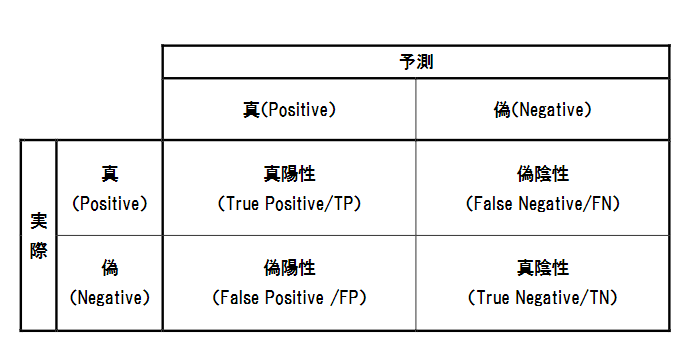
\includegraphics[scale=0.7]{fig7_CM.png}}}
    \caption{混同行列のモデル}
    \label{CM}
\end{figure}

\indent 図\ref{CM}にあるように,混同行列では,以下の4パターンが存在する.\\
\begin {itemize}
\item \textbf{真陽性(True Positive/TP)}:予測で陽性と判断され,実際に陽性である.
\item \textbf{真陰性(True Negative/TN)}:予測で陰性と判断され,実際に陰性である.
\item \textbf{偽陽性(False Positive/FP)}:予測で陽性と判断されたが,実際は陰性である.
\item \textbf{偽陰性(False Negative/FN)}:予測で陰性と判断されたが,実際は陽性である.
\end{itemize}

\indent これら4つのパターンの値から,さまざまな評価指数が算出されるので,以下に紹介していく.
\begin {itemize}

\item \textbf{正解率(Accuracy)}\\
\indent すべての予測のうち正しく分類できた割合を示す.高いほど性能が良い.\\
\indent メリット:直感的でわかりやすい.\\
\indent デメリット:PositiveとNegativeの出現の偏りが大きいデータには,不適切である.\\
\begin{equation*}
	Accuracy = \frac{TP+TN}{TP+FP+FN+TN}
\end{equation*}
\\
\item \textbf{適合率(Presision)}\\
\indent  陽性と予測したもののうち,実際に陽性である割合を示す.高いほど性能が良い.\\
\indent メリット:偽陽性FPを小さくすることを目標としており,誤って陽性と判断しては困る場合に有効.\\
\indent デメリット:偽陰性FNが多いことが問題になるケースでは推奨されない.\\
\begin{equation*}
	Precision = \frac{TP}{TP+FP}
\end{equation*}
\\
\item \textbf{再現率(Recall)}\\
\indent  取りこぼしなく陽性であるデータを正しく陽性であると予測した割合を示す.高いほど性能が良い.\\
\indent メリット:偽陰性FNを小さくすることを目標としており,誤って陰性と判断しては困る場合に有効.\\
\indent デメリット:偽陽性FPが多いことが問題になるケースでは推奨されない.\\
\begin{equation*}
	Recall = \frac{TP}{TP+FN}
\end{equation*}
\\
\item \textbf{F値}\\
\indent 再現率と適合率の\textbf{調和平均}である(調和平均とは,「逆数の平均の逆数」で定義されている).\\
\indent 一般的に,適合率と再現率はトレードオフの関係であり,再現率と適合率を一方に偏らせずに均等に評価したい場合にF値は適している.\\
\begin{equation*}
	F-measure = \frac{2\times Precison\times Recall}{Precision+Recall}
\end{equation*}
\end{itemize}

\vspace{10mm}
\indent 1章で挙げた例と同じく,他の企業に対して契約が成立するか成立しないかの予測と実績として,以下のような結果が得られたとする.\\
\begin{figure}[H]
    \centering
    \mbox{{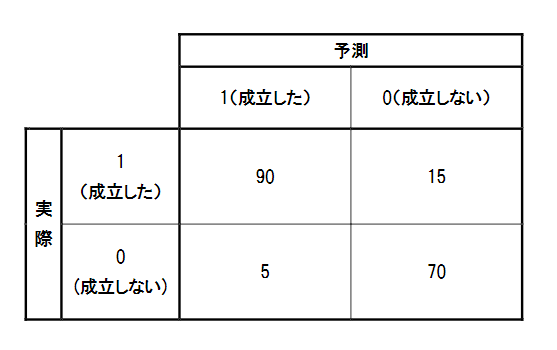
\includegraphics[scale=0.7]{fig7_CM_ex.png}}}
    \caption{営業データの予測による混合行列}
    \label{CM_ex}
\end{figure}

\indent このモデルに対して,上記の評価指数を計算すると,正解率:約89\%,適合率:約95\%,再現率:約86\%		,F値:0.89である.よって,適合率と再現率から,このモデルでは陽性と予測したものの信憑性はかなり高く,その反面実際に陽性であるものを陰性として予測してしまう可能性が少し高いことがわかる.\\

\section{まとめ}
\indent 今回のゼミでは,ロジスティック回帰の概要からモデル構築の方法と予測方法,そしてモデルの評価方法について紹介した.以下に要点を示す.\\
\begin{itemize}
\item ロジスティック回帰は二値分類を行う分類手法の一種.
\item モデル構築の際は\textbf{対数尤度}関数より\textbf{勾配降下法}の手法を用いて,最適な重み$\mathbm{w}$を求める.
\item 予測の際は,\textbf{シグモイド関数}を用いて確率的に分類する.
\item モデルの評価方法として{混同行列}紹介した.二値分類を行うモデルの評価として採用される評価モデルである.
\end{itemize}


\end{document}














